% Sezione per la macchina a stati
\begin{figure}[t]	
	\centering	
	{\includegraphics[width=\textwidth,keepaspectratio]
		{fsm.eps}}
	\caption{Macchina a stati finiti}
	\label{fsm} 
\end{figure}
\subsection{Macchina a stati finiti}

Per la gestione dei segnali di controllo \`e stata realizzata la macchina con 9 stati illustrata in Figura \ref{fsm}. Oltre a S0 si compone di 3 macrostati:
\begin{itemize}
	\item S1 + S2 + S3: Stati di inizializzazione;
	\item S4 + S5 + S6: Stati di analisi;
	\item S7 + S8: Stati di output. 
\end{itemize}
L'interazione degli stati con la pipeline \`e illustrata in Figura \ref{pipeline}.

\subsubsection{S0}
\textbf{S0} \`e lo stato iniziale e di reset, in cui il sistema rimane finch\'e \mbox{\texttt{i\_start} = 0}. Sono stati omessi dallo schema tutti i collegamenti da ogni stato che rappresentano la transizione per \texttt{i\_rst} = 1.

\subsubsection{Stati di inizializzazione: S1, S2, S3}
In \textbf{S1} viene inizializzato \texttt{regnext} e viene richiesto alla memoria l'indirizzo da codificare (poich\'e \texttt{mux\_nxt} = 0).

\textbf{S2} si occupa invece di caricare in \texttt{regin} l'indirizzo da codificare e richiedere l'indirizzo della prima Working Zone (ponendo a 1 \texttt{mux\_nxt}).

\textbf{S3} infine carica l'indirizzo della prima WZ in \texttt{regwz} e prepara l'esecuzione parallela con la pipeline.

\subsubsection{Stati di analisi: S4, S5, S6}
\textbf{S4} \`e il primo stato di elaborazione, con pipeline a regime; analizza l'indirizzo in \texttt{regin} e la WZ in \texttt{regwz}, finch\'e non trova la WZ di appartenenza (per cui il sistema passa in stato di output) o il registro \texttt{regnext} raggiunge la fine delle celle di memoria contenenti le Working Zones (e avviene la transizione verso S5).

\textbf{S5} \`e lo stato di elaborazione in cui non \`e pi\`u necessario leggere in memoria, quindi viene bloccato l'accesso agli indirizzi successivi al 7; le altre due linee di pipeline possono continuare se non \`e stata trovata la WZ corretta (altrimenti si passa in output).

\textbf{S6} \`e l'ultimo stato di elaborazione e consiste nel bloccare anche il caricamento in memoria mentre viene effettuata l'analisi dell'ultima WZ. Sia che la WZ analizzata contenga l'indirizzo sia che non lo riguardi, S6 evolve nello stato di output.

\subsubsection{Stati di Output: S7, S8}
\textbf{S7} permette di scrivere in memoria, in posizione 9, il risultato (controllato interamente da \texttt{is\_in}).

\textbf{S8} \`e l'ultimo stato di un'elaborazione; attiva i flag \texttt{o\_done} e \texttt{end\_reset}, quest'ultimo con funzione analoga a \texttt{i\_reset} per i registri. Infine, riporta il sistema allo stato iniziale quando \texttt{i\_start} torna a 0.

\subsubsection{Segnali di controllo e VHDL}
La codifica della macchina a stati \`e stata realizzata con due process, rispettivamente per gestire le transizioni (sia in casi normali che in caso di reset) e per attivare i segnali di controllo opportuni in base allo stato corrente (con un \texttt{case}); nelle due tabelle sottostanti sono riassunti i segnali attivi per ogni stato.
\begin{center}
	\begin{tabular}[width=\textwidth]{c|c c c|c c|c}
		  & o\_en & o\_we & o\_done & mux\_nxt & mux\_mem & end\_reset \\
		\hline
		S0 & 0 & 0 & 0 & 0 & 0 & 0 \\
		S1 & 1 & 0 & 0 & 0 & 0 & 0 \\
		S2 & 1 & 0 & 0 & 1 & 0 & 0 \\
		S3 & 1 & 0 & 0 & 1 & 0 & 0 \\
		S4 & 1 & 0 & 0 & 1 & 0 & 0 \\
		S5 & 1 & 0 & 0 & 1 & 1 & 0 \\
		S6 & 1 & 0 & 0 & 1 & 1 & 0 \\
		S7 & 1 & 1 & 0 & 0 & 1 & 0 \\
		S8 & 0 & 0 & 1 & 0 & 0 & 1 
	\end{tabular}
\end{center}
\begin{center}
	\begin{tabular}[width=\textwidth]{c|c c c c}
		 & regnext\_load & regin\_load & regwz\_load & regsub\_load \\
		\hline
		S0 & 0 & 0 & 0 & 0 \\
		S1 & 1 & 0 & 0 & 0 \\
		S2 & 1 & 1 & 0 & 0 \\ 
		S3 & 1 & 0 & 1 & 0 \\
		S4 & 1 & 0 & 1 & 1 \\
		S5 & 1 & 0 & 1 & 1 \\ 
		S6 & 1 & 0 & 0 & 1 \\
		S7 & 0 & 0 & 0 & 0 \\
		S8 & 0 & 0 & 0 & 0
	\end{tabular}
\end{center}